\documentclass{scrartcl}
\usepackage{lscape}
\usepackage{tikz}

\begin{document}
\begin{landscape}
\centering
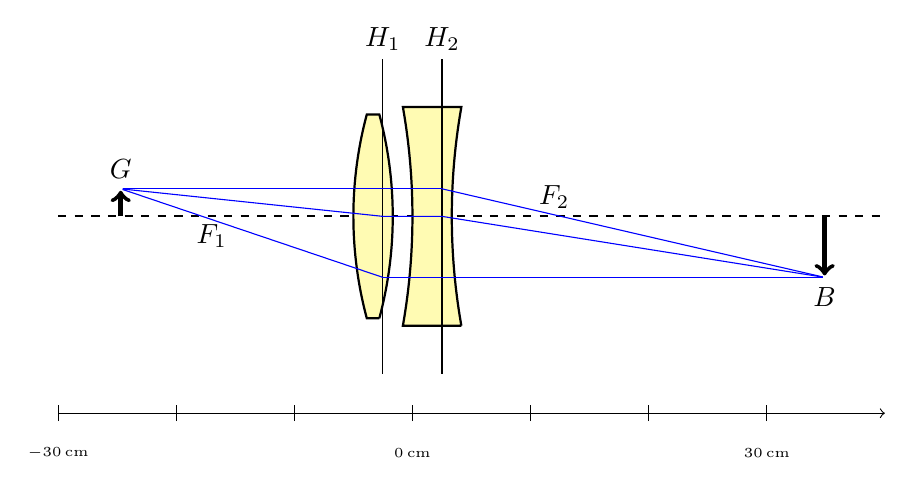
\begin{tikzpicture}[scale=0.5, inner sep=0]
\def\sx{0.3}

% Optische Achse
\draw[dashed, thick] (-30*\sx,0) -- (40*\sx,0);
% Koordinaten Nullpunkt
\draw (0,-0.2) -- (0,0.2);

% Konkave Linse
\def\xconv{0.5} % x-Koordinate
\draw[thick, fill=yellow!30] 
     ([shift=(190:16cm)]16.5+\xconv,0) arc (190:170:16cm)
     -- ([shift=(10:16cm)] -16.5+\xconv,0)
     arc (10:-10:16cm) 
     -- ([shift=(190:16cm)]16.5+\xconv,0);

% Konvexe Linse
\def\xconx{-1.5} % x-Koordinate
\draw[thick, fill=yellow!30] ([shift=(-15:10cm)]-9+\xconx,0) arc (-15:15:10cm)
 --([shift=(165:10cm)]10+\xconx,0) arc (165:195:10cm)
 --([shift=(-15:10cm)]-9+\xconx,0);

% Gegenstand (Pfeil)
\def\Gx{-24.7*\sx}
\def\Gy{0.7}
\node (G) at (\Gx,\Gy) {};
\draw[->, ultra thick] (\Gx,0) -- (G);%
\node (labG) at (\Gx,\Gy+0.5) {$G$};
% Bild (arrow)
\def\Bx{34.9*\sx}
\def\By{-1.55}
\node (B) at (\Bx,\By) {};
\draw[->, ultra thick] (\Bx,0) -- (B);
\node (labB) at (\Bx,\By-0.5) {$B$};

% Hauptebenen
\def\Hx{2.5*\sx}
\draw (\Hx,-4) -- (\Hx,4); % H1
\node (labH1) at (-\Hx,4.5) {$H_1$};
\draw (-\Hx,-4) -- (-\Hx,4); % H2
\node (labH2) at (\Hx,4.5) {$H_2$};

% Strahlen
% FokusG
\draw[color=blue] (G) -- (-\Hx,\By);
\draw[color=blue] (B) -- (-\Hx,\By);
% FokusB
\draw[color=blue] (G) -- (\Hx,\Gy);
\draw[color=blue] (B) -- (\Hx,\Gy);
%Central
\draw[color=blue] (G) -- (-\Hx,0) -- (\Hx,0)  -- (B);
               
% Label
%Fokus Punkte
\node (F1) at (-17*\sx,-0.5) {$F_1$};
\node (F2) at (12*\sx,0.5) {$F_2$};
% Koordinaten Nullpunkt
\def\cy{-5}
\draw[->] (-30*\sx,\cy) -- (40*\sx,\cy);
\draw (0,-0.2+\cy) -- (0,0.2+\cy);
\draw (10*\sx,-0.2+\cy) -- (10*\sx,0.2+\cy);
\draw (-10*\sx,-0.2+\cy) -- (-10*\sx,0.2+\cy);
\draw (20*\sx,-0.2+\cy) -- (20*\sx,0.2+\cy);
\draw (-20*\sx,-0.2+\cy) -- (-20*\sx,0.2+\cy);
\draw (30*\sx,-0.2+\cy) -- (30*\sx,0.2+\cy);
\draw (-30*\sx,-0.2+\cy) -- (-30*\sx,0.2+\cy);
\node (m30) at (-30*\sx,-1+\cy) {\tiny $-30\,\mathrm{cm}$};
\node (p30) at (30*\sx,-1+\cy) {\tiny $30\,\mathrm{cm}$};
\node (zero) at (0*\sx,-1+\cy) {\tiny $0\,\mathrm{cm}$};

% Gebogener Pfeil
%\draw[->, dashed] (9.5,18) .. controls (4,18) .. (3,11.65);
\end{tikzpicture}
\end{landscape}
\end{document}